\documentclass[10pt]{beamer}

% shrugs
\usepackage{graphicx}
\def\shrug{\texttt{\raisebox{0.75em}{\char`\_}\char`\\\char`\_\kern-0.5ex(\kern-0.25ex\raisebox{0.25ex}{\rotatebox{45}{\raisebox{-.75ex}"\kern-1.5ex\rotatebox{-90})}}\kern-0.5ex)\kern-0.5ex\char`\_/\raisebox{0.75em}{\char`\_}}}


%\usetheme[progressbar=frametitle]{metropolis}
\usepackage{appendixnumberbeamer}
\usepackage[font=scriptsize,labelfont=bf]{caption}
\usepackage{booktabs}
\usepackage[scale=2]{ccicons}
%%%%%%%%%%%%%%%%%%%%%%%%
\usepackage{minted}

%%%% Logo - https://tex.stackexchange.com/a/53783
\newif\ifplacelogo % create a new conditional
\placelogotrue
\logo{\ifplacelogo
\includegraphics[height=1.5cm]{images/FFT_Time_mage.jpg}\fi}

%%%%%%%%%%%%%%%%%%%%%%%%
\title[datetime]{datetime}
\subtitle{A Tale of Pythonic Woe}
\author{Dave Voutila}
\institute{
	voutilad@gmail.com \\
	https://github.com/voutilad \\
	@voutilad
}
\date{23 August 2017}

\begin{document}
\maketitle

\section{Who am I?}
\begin{frame}{Who am I?}
	\begin{columns}
		\begin{column}{0.5 \textwidth}
			\begin{itemize}
				\item Independent Software Consultant
				\item Start-up Advisor
				\item Specializing in
					\begin{itemize}
						\item Python \& Java development expertise
						\item Software go-to-market \& Sales
						\item Making PowerPoint slides
						\item Wasting time with \LaTeX
					\end{itemize}
			\end{itemize}
		\end{column}
		\begin{column}{0.5 \textwidth}
			\centering
			
\includegraphics[width=3cm]{images/sisu.png}
			\vspace{1cm}
			
\includegraphics[width=3cm]{images/ta.png}
		\end{column}
	\end{columns}
\end{frame}

\placelogofalse
\section{The Logo}
\begin{frame}{What's with the little people?}
	\begin{figure}
		\centering
		\includegraphics[width=5cm]{images/FFT_Time_Mage.jpg}
		\caption{Time Mages --- Final Fantasy Tactics}
	\end{figure}
\end{frame}

\placelogotrue

\section{Backstory}
\begin{frame}{Once upon a Github Issue...}
	\begin{figure}
		\centering
		
\includegraphics[width=6cm]{images/flaskask.png}
	\end{figure}
\begin{itemize}
\item Contributor to \textbf{Flask-Ask}, a Python Amazon Alexa framework.
\item Jumped on \textit{Issue 152: Flask Ask doesn't parse time stamp from Alexa properly...}
\item Things went downhill from there...
\end{itemize}
\end{frame}

\begin{frame}[fragile]{A Classic Github Issue}
	\begin{figure}
		\centering
		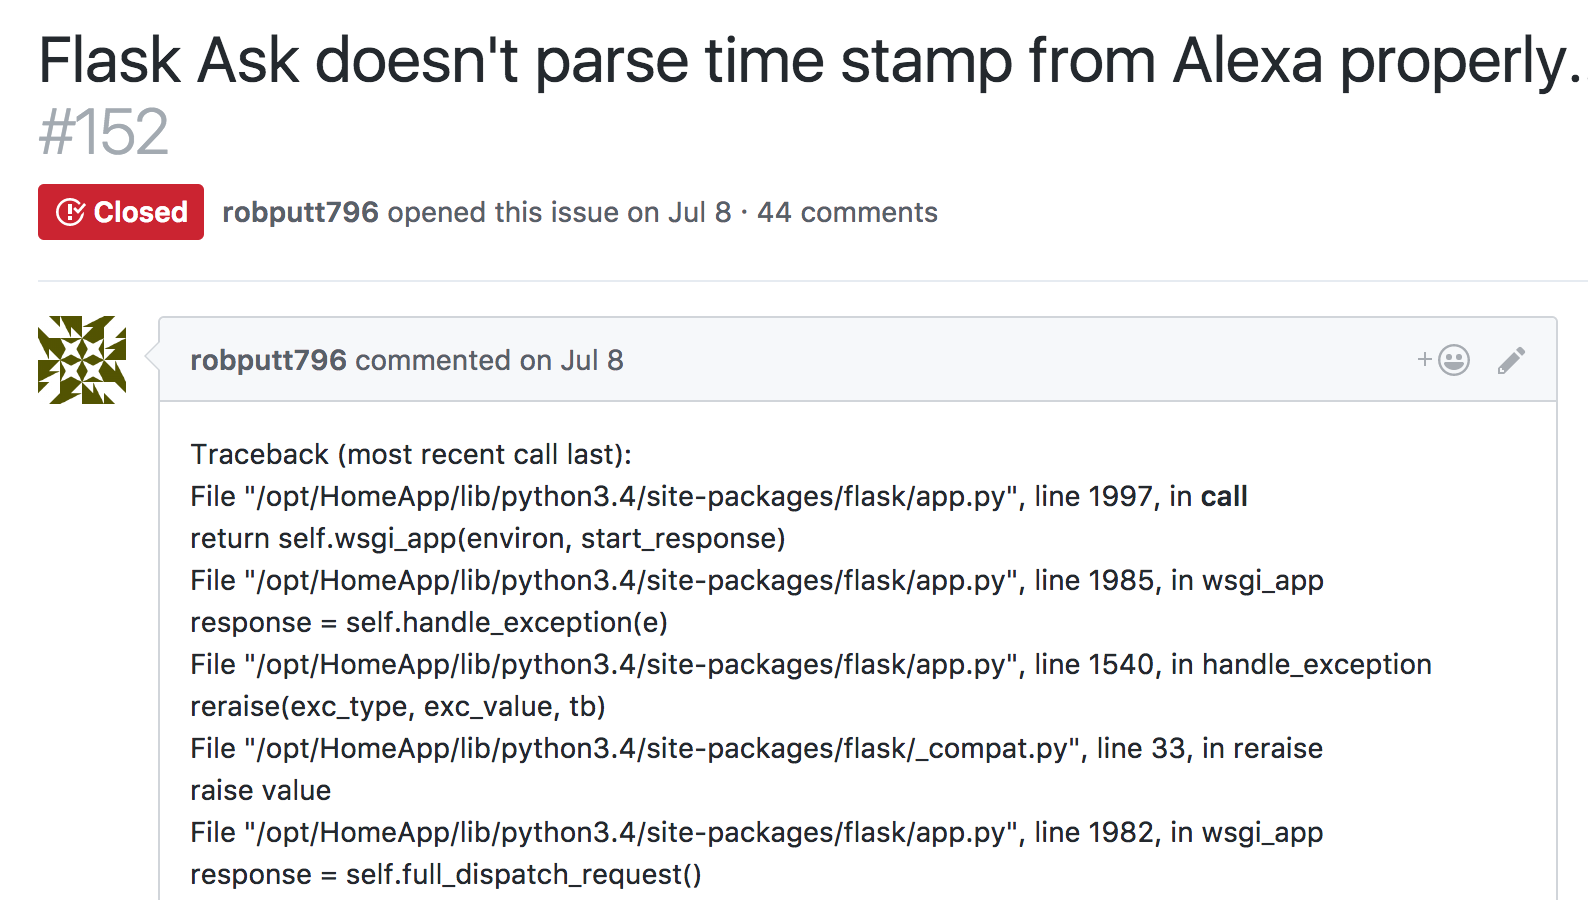
\includegraphics[width=\textwidth]{images/issue.png}
	\end{figure}
	\begin{itemize}
		\item Seriously...just a Traceback
		\item \mintinline{python}{AttributeError: 'int' object has no attribute 'split'}
	\end{itemize}
\end{frame}

\begin{frame}[fragile]{The Offending Code}
	\begin{minted}[linenos=false]{python}
timestamp = aniso8601.parse_datetime(
	alexa_request_payload['request']['timestamp']
)
	\end{minted}
	\begin{itemize}
		\item \texttt{aniiso8601} --- ISO-8601 parsing library
		\item Trying to de-reference items in the Alexa JSON
		\item \texttt{aniiso8601} is not happy with the value it's given
		\item So if it's not a String, what is it?
	\end{itemize}
\end{frame}

\section{The Investigation}
\begin{frame}{RTFM}
		\begin{itemize}
			\item Let's see what Amazon's documentation says about "timestamps":
		\end{itemize}
			\begin{figure}
				\centering
				\fbox{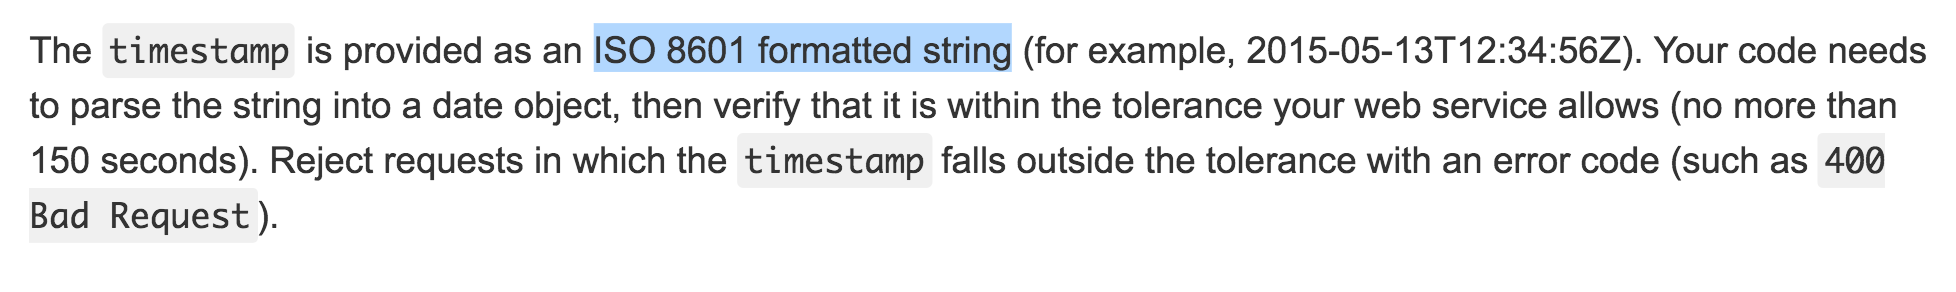
\includegraphics[width=\textwidth]{images/docs.png}}
				\caption{\url{https://developer.amazon.com/public/solutions/alexa/alexa-skills-kit/docs/developing-an-alexa-skill-as-a-web-service\#timestamp}}
			\end{figure}
		\begin{itemize}
			\item Ok, so we \textit{should} get something like: \mintinline{python}{"2009-02-13T23:31:30Z"}
	\end{itemize}
\end{frame}

\begin{frame}{Alexa}
\begin{center}
	\begin{figure}
		\centering
		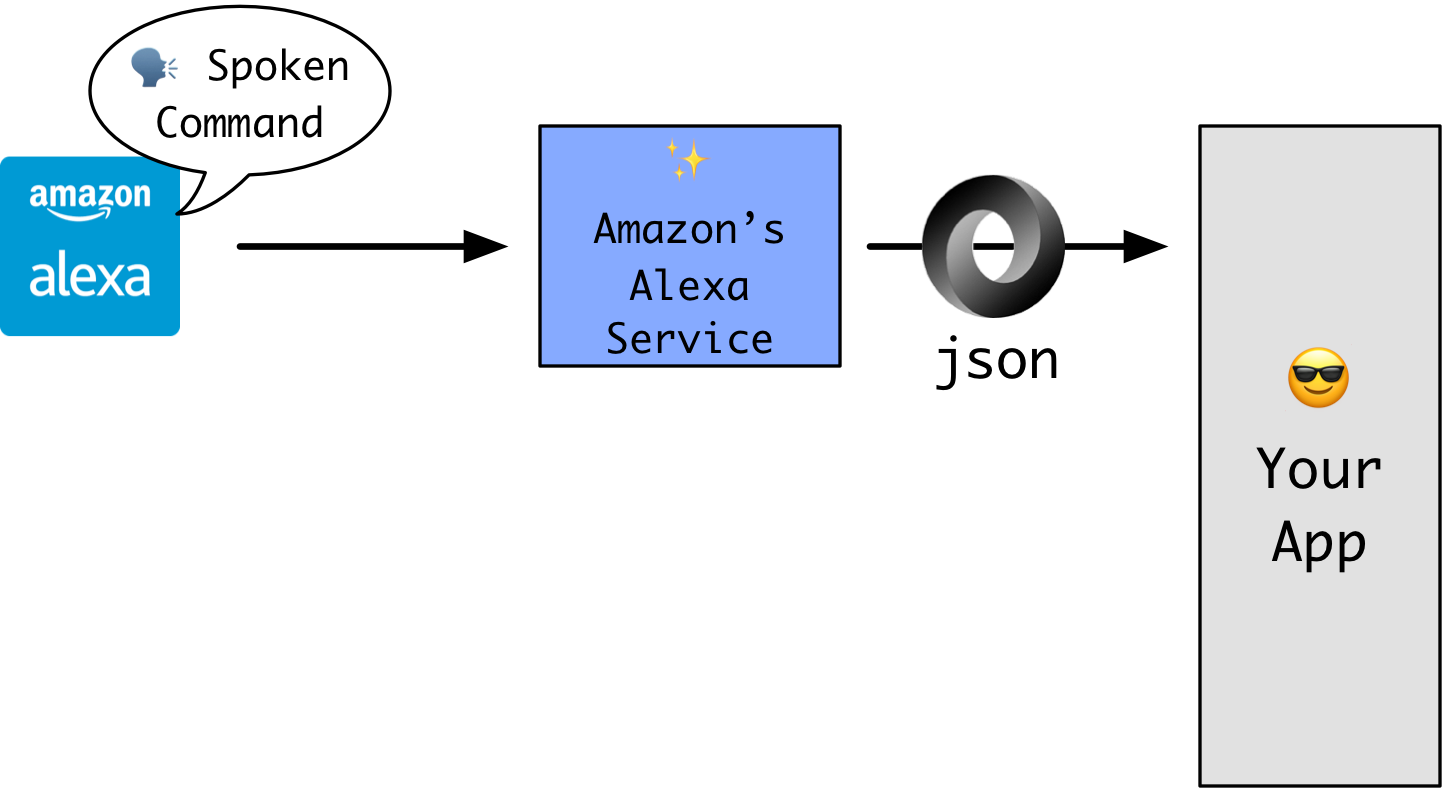
\includegraphics[width=\textwidth]{./images/alexa-flow-01.png}
		\caption{super simple Alexa architecture}
	\end{figure}
\end{center}
\end{frame}

\begin{frame}{Amazon Lies}
\begin{center}
	\begin{figure}
		\centering
		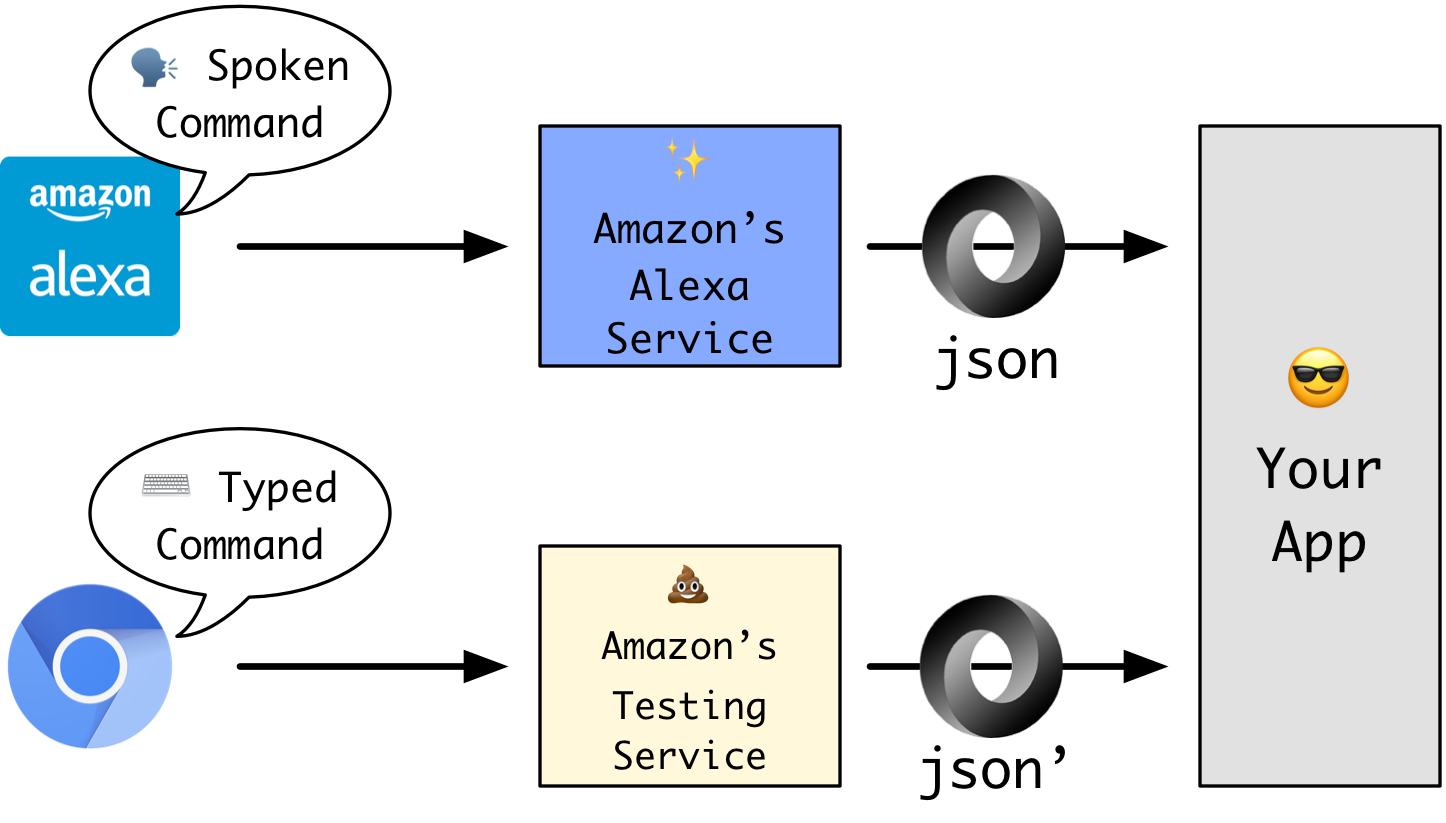
\includegraphics[width=\textwidth]{./images/alexa-flow-02.png}
		\caption{json $\protect\neq$ json'}
	\end{figure}
\end{center}
\end{frame}

\begin{frame}{Good Agent Cooper vs. Evil Agent Cooper}
	\begin{itemize}
		\item One of these things is not like the other...
	\end{itemize}
	\begin{columns}
		\begin{column}{0.5 \textwidth}
			\inputminted[fontsize=\small,frame=single,framesep=2mm,linenos=false,breaklines]{javascript}{src/good.json}
		\end{column}
		\begin{column}{0.5 \textwidth}
			\inputminted[fontsize=\small,frame=single,framesep=2mm,linenos=true,breaklines]{javascript}{src/bad.json}
		\end{column}
	\end{columns}
	\begin{itemize}
		\item So, that lovely integer is the epoch time in milliseconds.
		\item ...for UTC? \shrug
	\end{itemize}
\end{frame}

\section{Solving the Mystery}
\begin{frame}{First Attempt}
	\begin{itemize}
		\item Wanted a simple solution to handle both \texttt{string}s and \texttt{int}s
		\item If fails to parse, handle the \texttt{AttributeError} and assume an int
	\end{itemize}
	\begin{figure}
		\centering
		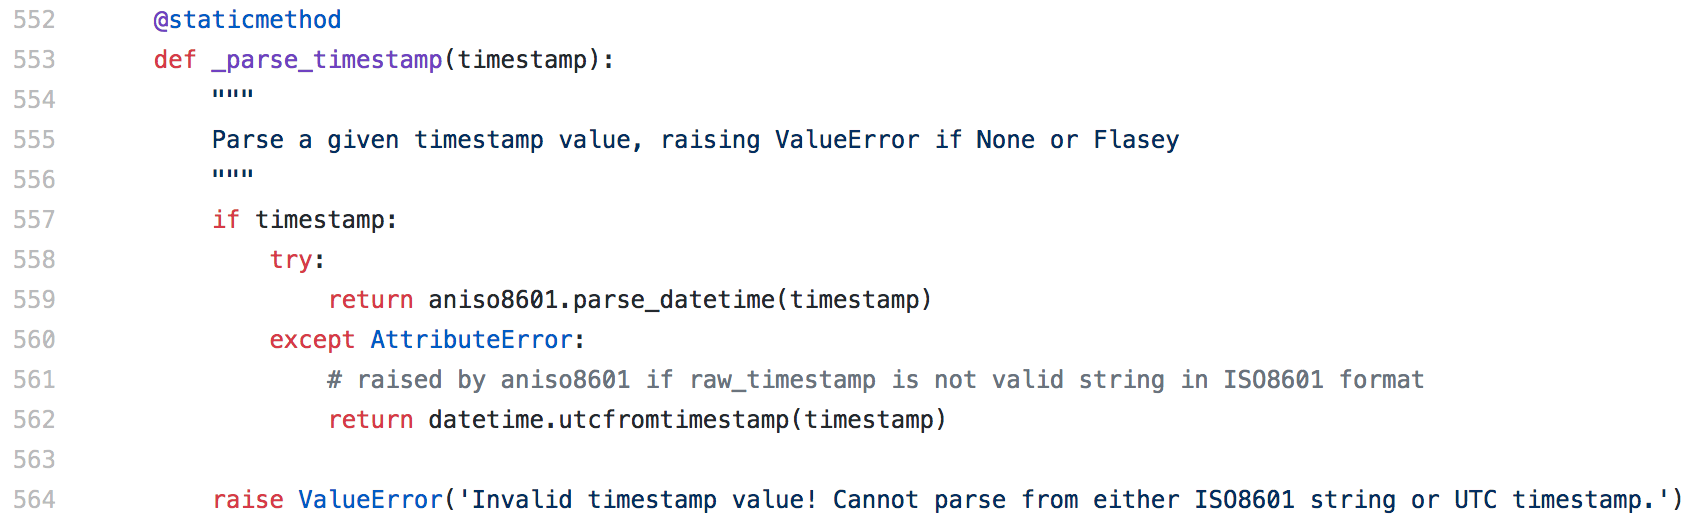
\includegraphics[width=\textwidth]{images/commit1.png}
		\caption{core.py --- 3240a43c4dce6b1cf45754c2d8ac82a7f9c150a6}
	\end{figure}
\end{frame}

\renewcommand{\arraystretch}{1.5}
\begin{frame}{Lesson 1: Python's a bit Odd (as is C\#)}
	\begin{itemize}
		\item Well...it's not just Python, but precision is key.
	\end{itemize}
	\begin{center}
		\begin{tabular}{ c c c }
			Language & Example & Precision \\
			\hline
			Go & \mintinline{go}{time.Time} & nanoseconds \\
			Java & \mintinline{java}{java.lang.System.getNanos()} & nanoseconds \\
			C\# & \mintinline{csharp}{DateTime.Ticks} & \(\frac{1}{10}\) microseconds \\
			Javascript & \mintinline{javascript}{Date.now()} & milliseconds \\
			Python & \mintinline{python}{time.time()} & microseconds
		\end{tabular}
	\end{center}
	\begin{itemize}
		\item But wait, there's more!
	\end{itemize}
\end{frame}

\begin{frame}{Nobody will live to see 41091 AD anyways...}
	\begin{figure}
		\centering
		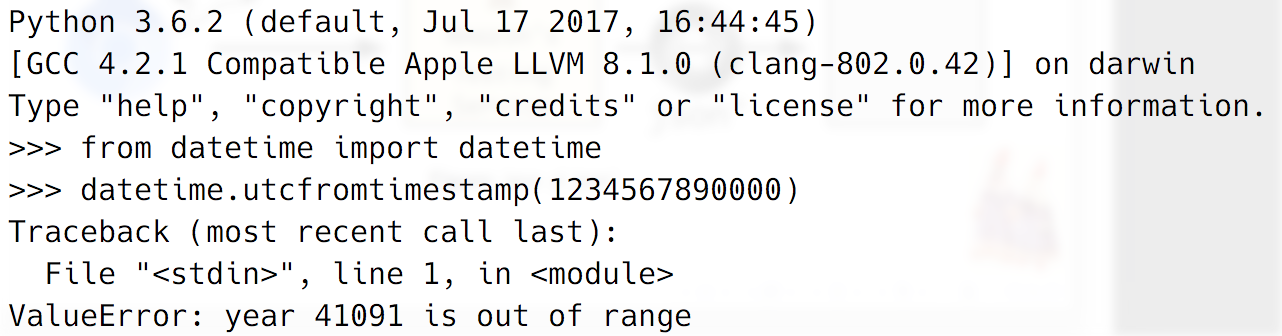
\includegraphics[width=\textwidth]{images/valueerror.png}
	\end{figure}
	\begin{itemize}
		\item Ok, so if Amazon sends milliseconds, lets scale it.
	\end{itemize}
\end{frame}

\section{Second Attempt}
\begin{frame}{Second Attempt}
	\begin{itemize}
		\item So turns out Python uses \textbf{microseconds}
		\item Try this again, but now while scaling the value...
	\end{itemize}
	\begin{figure}
		\centering
		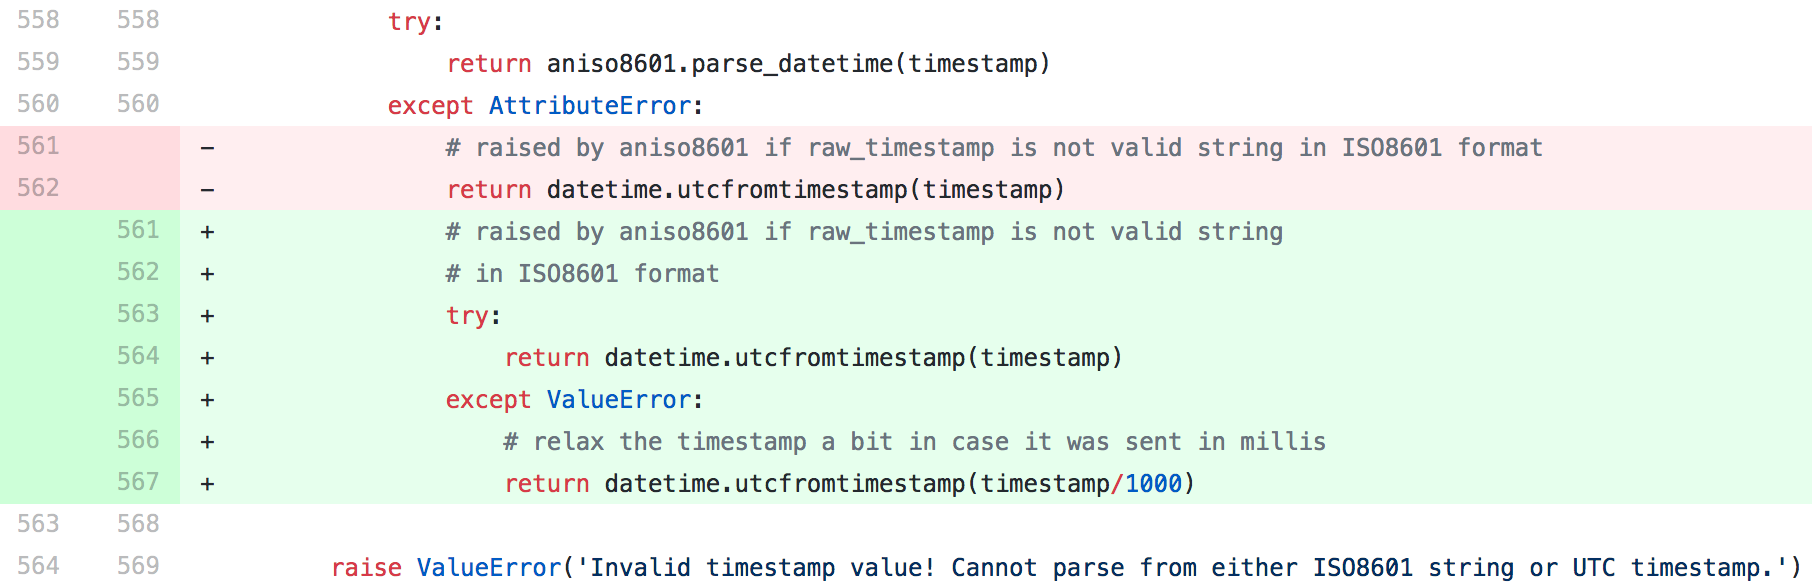
\includegraphics[width=\textwidth]{images/commit2.png}
		\caption{core.py --- 17ba43a60fc4e0b91f00d596aa3cfc78c81771a9}
	\end{figure}
\end{frame}

\begin{frame}{Never test on just your machine!}
	\begin{itemize}
		\item Windows: what the heck \shrug
	\end{itemize}
	\begin{figure}
		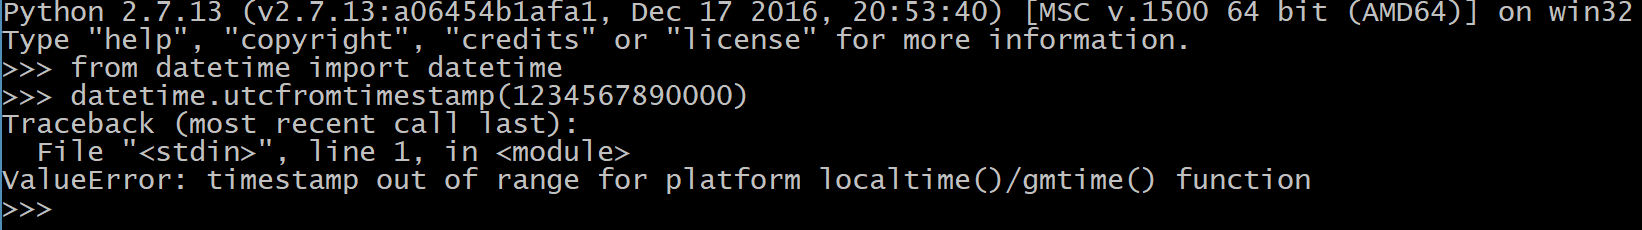
\includegraphics[width=\textwidth]{images/windows-py27.png}
		\vspace{1cm}
		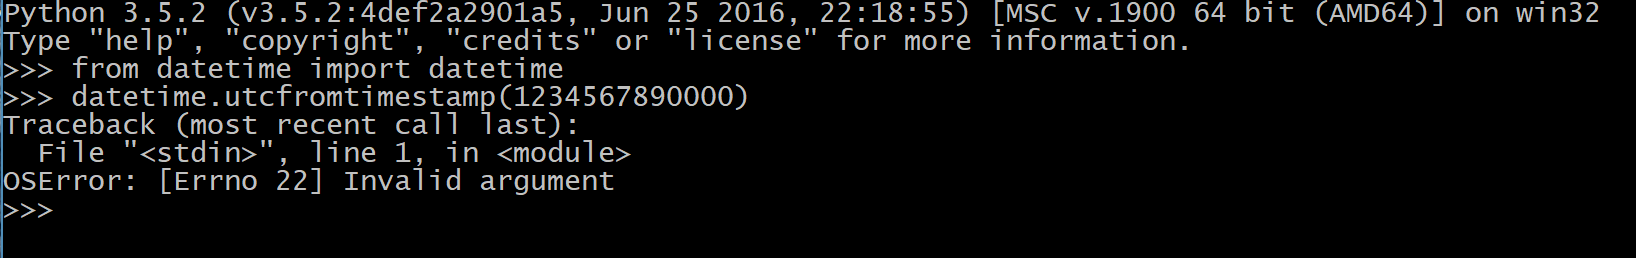
\includegraphics[width=\textwidth]{images/windows-py35.png}
	\end{figure}
\end{frame}

\begin{frame}{Lesson 2: Python Time Handling is System Dependent}
	\begin{columns}
		\begin{column}{0.5 \textwidth}
			\begin{itemize}
				\item Python's \texttt{time} module is all native \texttt{C}
				\item \texttt{datetime} uses \texttt{time}
					\begin{itemize}
						\item \texttt{datetime} is pure Python
						\item A leaky abstraction
					\end{itemize}
				\item Calls to \texttt{datetime.utcfromtimestamp()} trigger the code on the right
				\item \textbf{Hint} --- this will be a factor
			\end{itemize}
		\end{column}
		\begin{column}{0.5 \textwidth}
			\begin{figure}
				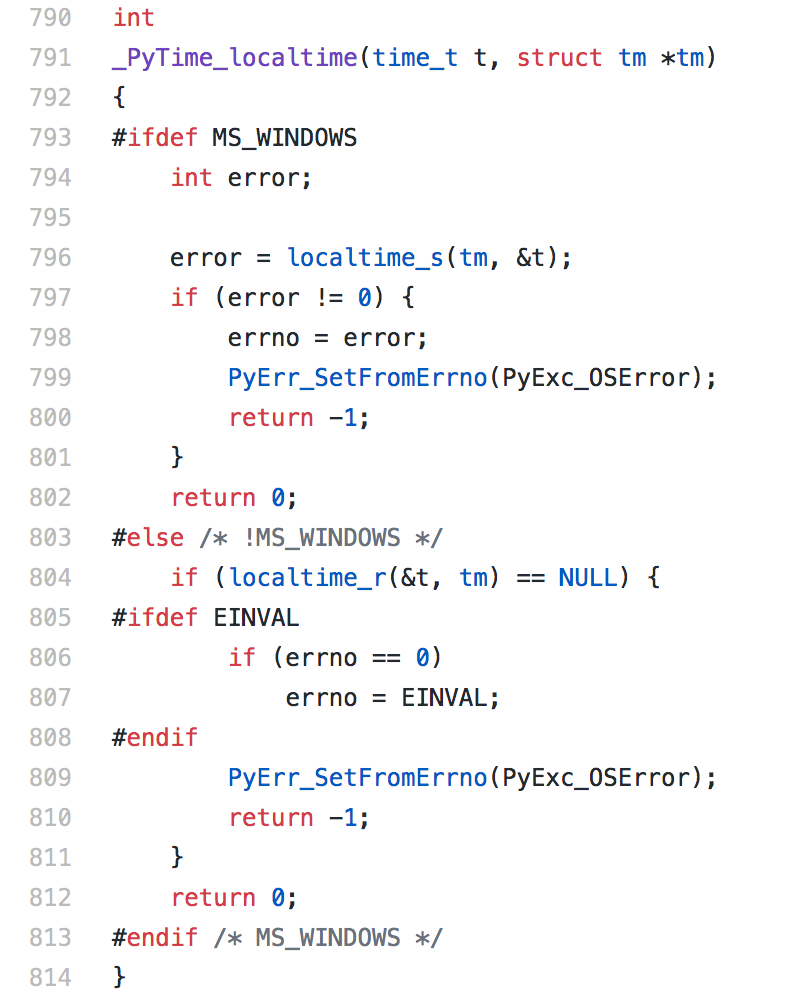
\includegraphics[width=0.9\columnwidth]{images/rabbithole.png}
				\caption{pytime.c}
			\end{figure}
		\end{column}
	\end{columns}
\end{frame}

\section{Third Attempt}
\begin{frame}{Third Attempt}
	\begin{itemize}
		\item I give up!
	\end{itemize}
	\begin{figure}
		\centering
		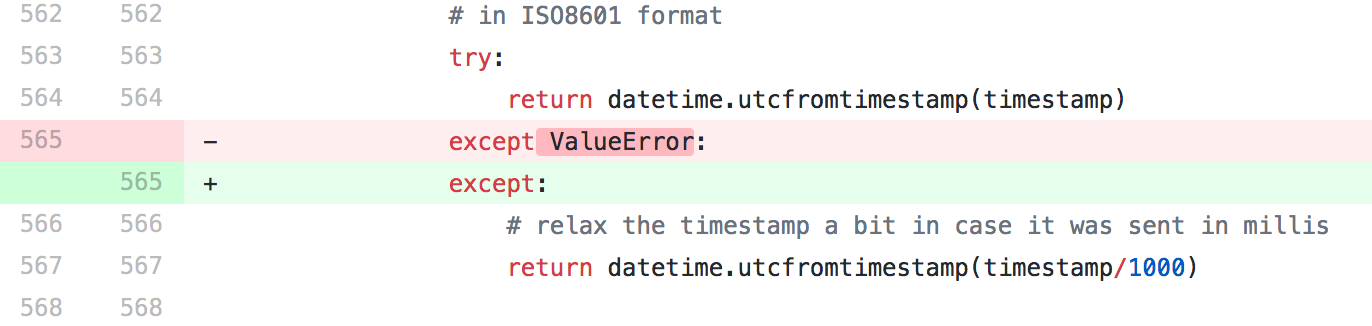
\includegraphics[width=\textwidth]{images/commit3.png}
		\caption{core.py --- 8de0db687cb6ff28d7b9bed251480060b01d5736}
	\end{figure}
\end{frame}

\section{The End}
\begin{frame}{Happy ending?}
	\begin{itemize}
		\item Case closed! I guess it works now.
		\item But...Python still thinks none of us will like to see 10000AD :-(
	\end{itemize}
	\begin{figure}
		
\includegraphics[width=\textwidth]{images/eol.png}
		\caption{CPython's \_datetimemodule.c}
	\end{figure}
\end{frame}
\end{document}

